\documentclass[a4, 14pts]{seminar}
\usepackage[dvips]{pstcol}
\usepackage{semcolor}
\usepackage{sem-page}
\usepackage{slidesec}
\input{seminar.bug}
\input{seminar.bg2}
\usepackage{semhelv}
\usepackage{subfigure}
\usepackage[latin1]{inputenc}
\usepackage[T1]{fontenc}
\usepackage{times}
\usepackage{longtable,array,enumerate}


\usepackage{multicol}

\usepackage[intlimits,sumlimits,namelimits]{amsmath}
\usepackage{amsmath}

\usepackage{amssymb}
\usepackage[mathscr]{eucal}
\usepackage{mathrsfs}
\usepackage{amsthm}
\usepackage{amsfonts}
\usepackage{amsmath}

\usepackage[dvips]{graphicx}
\usepackage{epsf}
\usepackage{epsfig}
\usepackage{fancyhdr}
\usepackage{layout}

\usepackage[french]{babel}
\usepackage[T1]{fontenc}
\usepackage[latin1]{inputenc}

\usepackage{url}
\usepackage{xspace}

\DeclareMathOperator{\sign}{sign}


\newtheorem{corollary}{Corollaire}[section]
\newtheorem{definition}[corollary]{D\'{e}finition}
\newtheorem{equations}[corollary]{Equations}
\newtheorem{example}[corollary]{Exemple}
\newtheorem{lemma}[corollary]{Lemme}
\newtheorem{proposition}[corollary]{Proposition}
\newtheorem{remark}[corollary]{Remarque}
\newtheorem{theorem}[corollary]{Th\'{e}or\`{e}me}
	    %%% The above 7 commands are used in the following way:
	    %%% The definition environment, for example, is created by
	    %%% \begin{definition}\label{xxx}. . .\end{definition}
\newcommand{\mylabel}[1]{\label{#1}
			\ifx\undefined\stillediting
			\else \fbox{$#1$}\fi }
\newcommand{\BE}{\begin{equation}}
\newcommand{\BEQ}[1]{\BE\mylabel{#1}}
\newcommand{\EEQ}{\end{equation}}
\newcommand{\rfb}[1]{\mbox{\rm
	      (\ref{#1})}\ifx\undefined\stillediting\else:\fbox{$#1$}\fi}
\newcommand{\half}   {{\frac{1}{2}}}
\newenvironment{matr}[1]{\left[ \begin{array}{#1}}{\end{array}	\right]}

\newfont{\Blackboard}{msbm10 scaled 1200}
\newcommand{\bl}[1]{\mbox{\Blackboard #1}}
\newfont{\roma}{cmr10 scaled 1200}

\newcommand{\propp}{{\hskip -2.2mm{\bf .}\hskip 3mm}}

\newcommand{\ovra}{\overrightarrow}
	    % fin des commandes de Marius

\fancyhf{}
\renewcommand\headrulewidth{0.2mm}
\renewcommand\footrulewidth{0.2mm}


\newcommand{\R}{\mathbb{R}}
\newcommand{\C}{\mathbb{C}}
\newcommand{\N}{\mathbb{N}}
\newcommand{\Z}{\mathbb{Z}}

\newcommand{\ROT}{{\text{Rot}}}
\newcommand{\Rot}{\vec{\text{Rot}}}
\newcommand{\rot}{\vec{\text{rot}}}

\newcommand{\dsp}{\displaystyle}

\usepackage{mathtools}
\DeclareMathOperator{\Mat}{Mat}
\DeclarePairedDelimiter{\diagfences}{(}{)}
\newcommand{\diag}{\operatorname{diag}\diagfences}
\newcommand\bigzero{\makebox(0,0){\text{\huge0}}}
\newcommand{\E}{\mathrm{E}}
\newcommand{\Var}{\mathrm{Var}}
\newcommand{\Cov}{\mathrm{Cov}}

\newcommand\eads{\textsf{}\xspace}
\newcommand\eadsccr{\textsf{}\xspace}

\fancyhead[L]{\theslideheading}
\fancyhead[R]{\textcolor{blue}{\eadsccr \thepage }}
\fancyfoot[R]{\textcolor{blue}{}}
\fancyfoot[L]{\textcolor{blue}{}} %% today
\renewcommand\headwidth{\textwidth}
\autoslidemarginstrue

\newslideframe{%
	      myscshadow}[\SemcolorFrameOps
	      \psset{shadowcolor=green}]{\psshadowbox{#1}}
\newcommand{\ud}{\mathrm{d}}

\newcommand{\ds}{\displaystyle}
\slideframe{myscshadow}
\setlength\slideframewidth{.5pt}
\setlength\footskip{1cm}
\setlength\headsep{1cm}

	    %\renewcommand\makeslideheading[1]{\par
	    %   \framebox{\theslidesection. #1}\par
	    %}
	    %\renewcommand\makeslidesubheading[1]{\par
	    %   \leavevmode\hspace*{1cm}%
	    %   \alph{slidesubsection}. #1\par
	    %}

\definecolor{Pink}{rgb}{1.,0.,0.2}
\definecolor{Mygreen}{rgb}{0.3,0.7,0.6}

\renewcommand\makeslideheading[1]{\par
	      \fcolorbox{black}{Mygreen}{\color{yellow}\theslidesection. #1}\par
	    }
\renewcommand\makeslidesubheading[1]{\par
	      \leavevmode\hspace*{1cm}%
	      \textcolor{Mygreen}{\alph{slidesubsection}. #1}\par
	    }

\makeatletter
\renewcommand\slide@contents{\par
	      \begin{center}
	\Large \bfseries\textcolor{blue}{Plan}
	      \end{center}
	      \def\l@slide##1##2##3{%
		\@undottedtocline{1}{1.5em}{2.3em}{\slidenumberline{##1.}{##2}}{}}%
	      \def\l@subslide##1##2##3{%
		\@undottedtocline{1}{1.5em}{3.3em}{\slidenumberline{\@alph{##1})}{##2}}{}}%
	      \@startlos
	    }
\makeatother

\slideframe{none}
	    %\XgrDefinitFormat{*}{line=0,mark=0,ll=1}
	    %\XgrDefinitFormat{pr}{}
	    %\XgrDefinitFormat{ks}{line=-1,mark=8,ll=0.4}
\begin{document}
\slidepagestyle{fancy}
	    %%%%%%%%%%%%%%%%%%%%%%%%%%%%%%%%%%%%%%%%%%%%%%%%%%%%%%%%%%%%%%%%%%%%%%%%%%%
\begin{slide}
\thispagestyle{plain}
\begin{center}
\textcolor{blue}{\huge  Trading sovereign debt futures}\\
\textcolor{blue}{\huge  Ravenpack news based machine learning signal}\\
\vspace{0.25 cm}
\textbf{DUPREY Stefan}\\
\small{\textbf{}\\ 

	    }
	    %\eadsccr
\end{center}
\end{slide}
	    %%%%%%%%%%%%%%%%%%%%%%%%%%%%%%%%%%%%%%%%%%%%%%%%%%%%%%%%%%%%%%%%%%%%%%%%%%
	    %%%%%%%%%%%%%%%%%%%%%%%%%%%%%%%%%%%%%%%%%%%%%%%%%%%%%%%%%%%%%%%%%%%%%%%%%%%
	    {\small{
\begin{slide}
\slidecontents
\renewcommand\theslideheading{Plan}
\end{slide}

%%%%%%%%%%%%%%%%%%%%%%%%%%%%%%%%%%%%%%%%%%%%%%%%%%%%%%%%%%%%%%%%%%%%%%%%%%%
%%%%%%%%%%%%%%%%%%%%%%%%%%%%%%%%%%%%%%%%%%%%%%%%%%%%%%%%%%%%%%%%%%%%%%%%%%%
{\small{
\begin{slide}
\slideheading{Building our pair trading signal}
Our ML algorithm outputs us with two predictions : the return for the first bond future $x_1$ and the return for the second bond
future return $x_2$, both for the same chosen rebalancing time period. We want to build our weights with the following properties, where T is a threshold parameter to limit our spread exposure $0<T<1$.
$T$ might also be seen as a guardrail when one of our prediction has low confidence : $x_1$ or $x_2$ is near zero.
\begin{equation}
\begin{displaystyle}
\begin{cases}
\left|  \omega_1 + \omega_2\right|=1\\
\sign(\omega_1) = \sign(x_1)\\
\sign(\omega_2) = \sign(x_2)\\
\frac{\omega_1}{\omega_2}=\frac{x_1}{x_2}\\
\text{if } \omega_1 + \omega_2 =1, \text{ then } \max(\omega_1,\omega_2) \leq 1+T\\
\text{if } \omega_1 + \omega_2 =-1, \text{ then } \min(\omega_1,\omega_2) \geq -1-T
\end{cases}
\end{displaystyle}
\end{equation}
\end{slide}
\begin{slide}
{\footnotesize
\slideheading{Weights expression}
\begin{equation}
\begin{displaystyle}
\begin{cases}
x_1 > 0, x_2 > 0 \begin{cases}  \omega_1=\frac{x_1}{x_1+x_2},\ \omega_2=\frac{x_2}{x_1+x_2}  \\ \omega_1+\omega_2=1,\ 0<\omega_1<1,\ 0<\omega_2<1    \end{cases} \\
x_1 < 0, x_2 < 0 \begin{cases}  \omega_1=-\frac{x_1}{x_1+x_2},\ \omega_2=-\frac{x_2}{x_1+x_2}  \\ \omega_1+\omega_2=-1,\ -1<\omega_1<0,\ -1<\omega_2<0    \end{cases} \\
x_1 < 0, x_2 > 0, \left|x_1\right| > x_2 \begin{cases}  \omega_2=\min(-\frac{x_2}{x_1+x_2},T),\ \omega_1=-1-\omega_2   \\ -1-T<\omega_1<-1,\ 0<\omega_2<T    \end{cases} \\
x_1 < 0, x_2 > 0, \left|x_1\right| < x_2 \begin{cases}  \omega_1=\max(\frac{x_1}{x_1+x_2},-T),\ \omega_2=1-\omega_1  \\ -T<\omega_1<0,\ 1<\omega_2<1+T    \end{cases} \\
x_1 > 0, x_2 < 0, \left|x_2\right| > x_1 \begin{cases}  \omega_1=\min(-\frac{x_1}{x_1+x_2},T),\ \omega_2=-1-\omega_1   \\ 0<\omega_1<T,\ -1-T<\omega_2<-1     \end{cases} \\
x_1 > 0, x_2 < 0, \left|x_2\right| < x_1 \begin{cases}  \omega_2=\max(\frac{x_2}{x_1+x_2},-T),\ \omega_2=1-\omega_1  \\ 1<\omega_2<1+T,\ -T<\omega_2<0    \end{cases} 
\end{cases}
\end{displaystyle}
\end{equation}
}
\end{slide}
\begin{slide}
\slideheading{Visualizing the confidence threshold}
\begin{center}
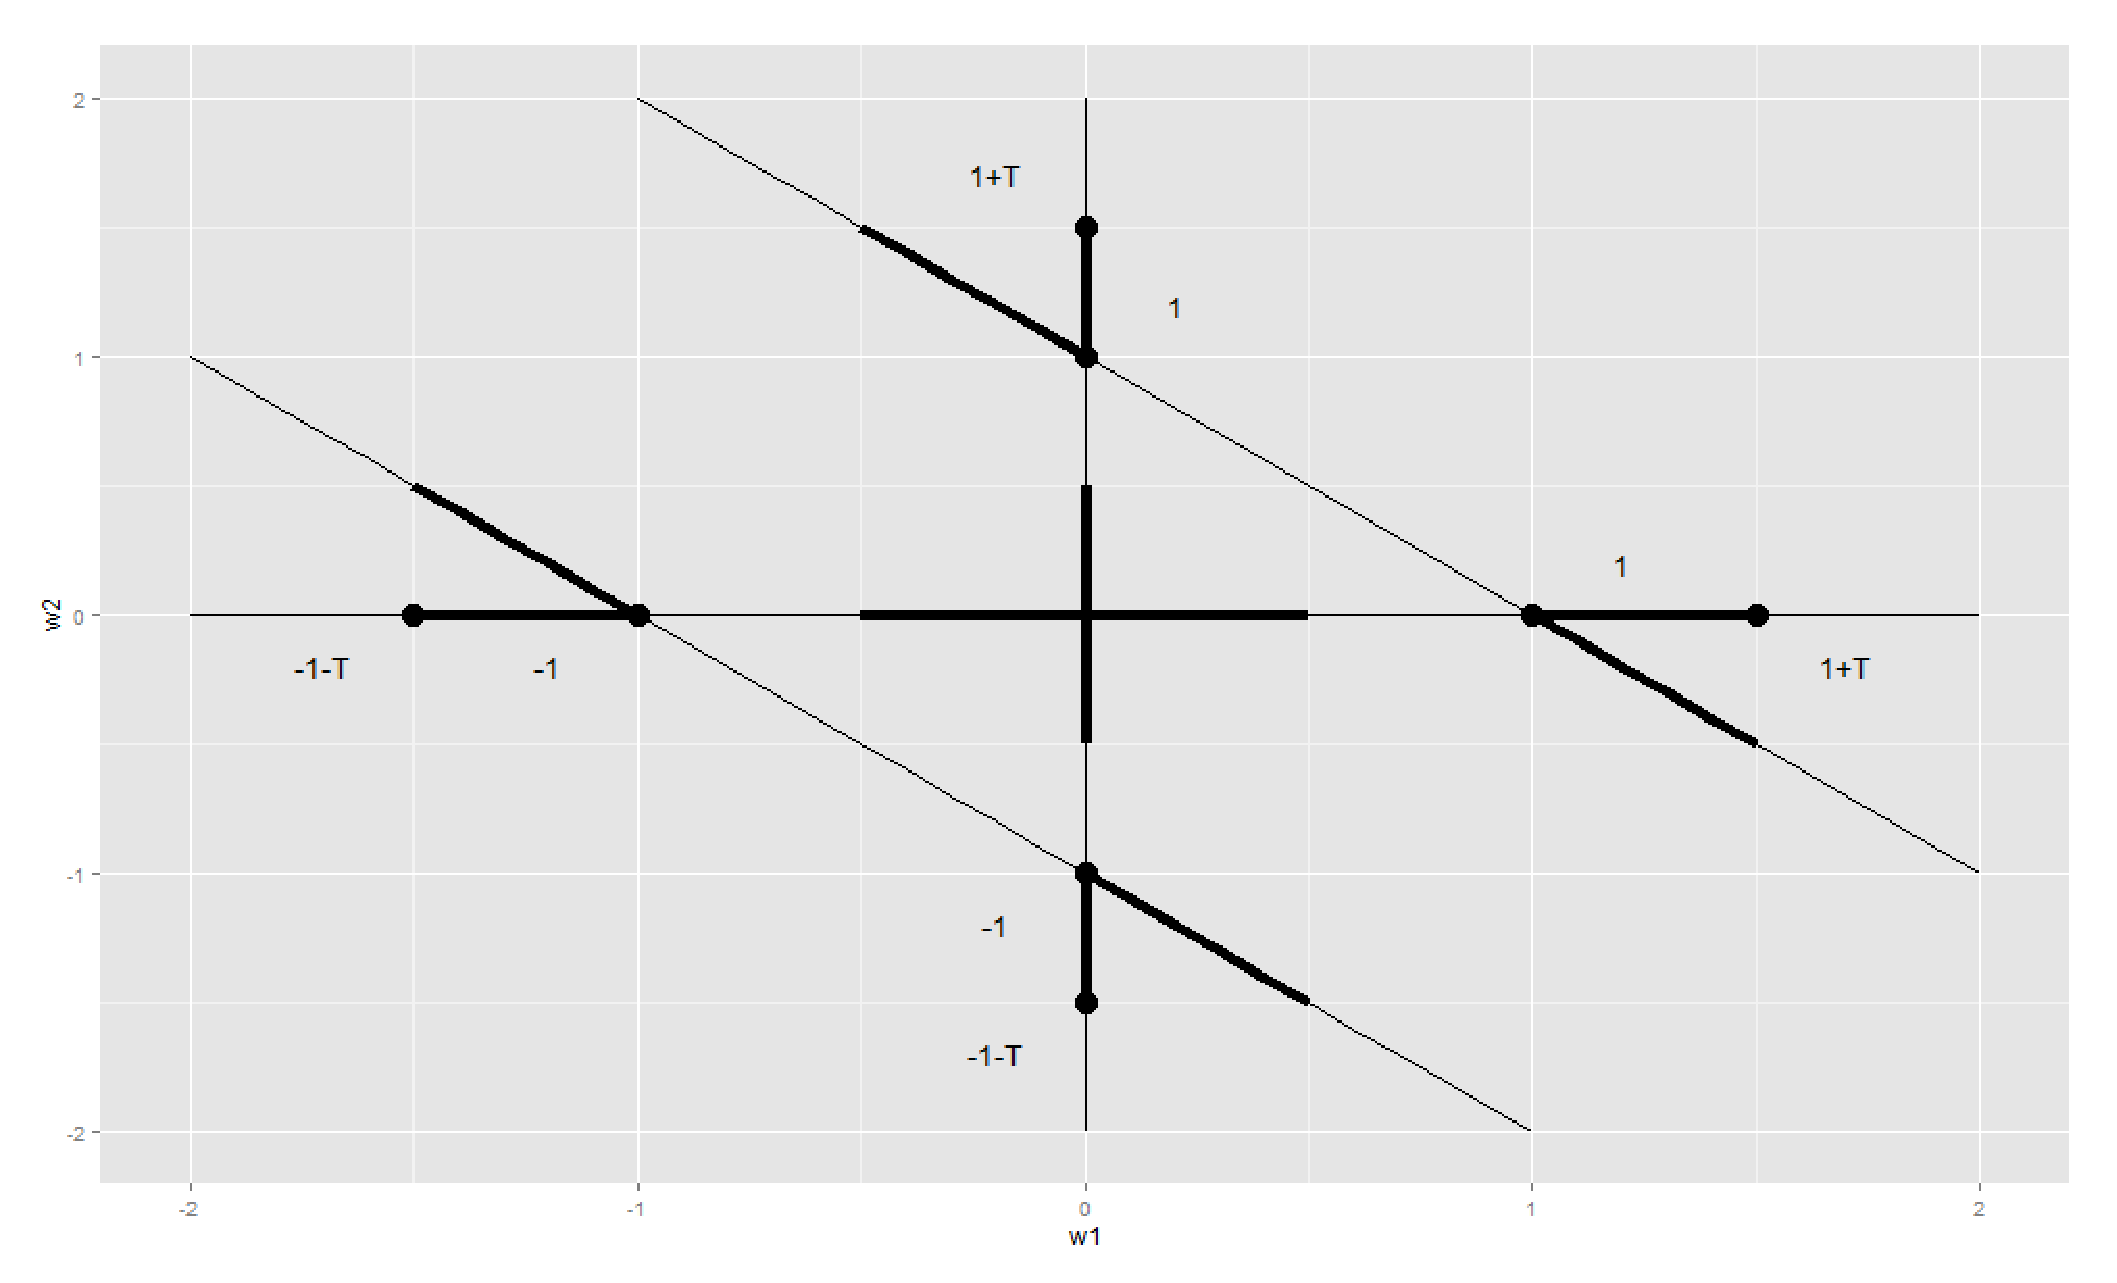
\epsfig{file=my_leveraged_weights.eps,height=6cm,width=6cm}
\end{center}
\end{slide}
\begin{slide}
\slideheading{Devising a sovereign debt basket strategy with the United States as a pivot}
The returns for each pair trading strategy against US. US is always traded first.
\begin{equation}
\begin{displaystyle}
\begin{cases}
\omega_{US/EU}R_{US}+\omega_{EU}R_{EU} \\
\omega_{US/UK}R_{US}+\omega_{UK}R_{UK} \\
\omega_{US/JP}R_{US}+\omega_{JP}R_{JP} \\
\end{cases}
\end{displaystyle}
\end{equation}
Equally weighted mix of each trading pair with US as pivot :
\begin{equation}
\frac{\left(\omega_{US/EU}+\omega_{US/UK}R +\omega_{US/JP}\right)}{3}R_{US} + \frac{\omega_{EU}}{3} R_{EU}+ \frac{\omega_{UK}}{3} R_{UK}+ \frac{\omega_{JP}}{3} R_{JP}
\end{equation}
\end{slide}
\end{document}
